\documentclass{article}

%%Configura??es padr?o

\usepackage{indentfirst}
\usepackage[brazilian]{babel}
\usepackage[utf8]{inputenc}
\usepackage{graphicx}
\usepackage[a4paper]{geometry}
\pagestyle{headings}
\usepackage[round]{natbib}
\usepackage{caption}
\usepackage[nottoc]{tocbibind}
\usepackage{pdfpages}

%%Estilo PUC

\geometry{left=3cm}
\geometry{right=4cm}
%\geometry{top=2.5cm}
%\geometry{bottom=2.5cm}
%\geometry{textheight=24.7cm}
\geometry{textwidth=13.5cm}

\setlength{\topmargin}{1cm}
%\setlength{\headsep}{10pt}
%\renewcommand{\footskip}{2.5cm}
%\setlength{\headheight}{1cm}
%\setlength{\textwidth}{13.5cm}
%\setlength{\marginparsep}{3cm}
\renewcommand{\baselinestretch}{1.5}
%\setlength{\marginparwidth}{0pt}
%\setlength{\voffset}{-1in}
%\setlength{\hoffset}{-0.5cm}
\parindent 1cm

%%Depura??o

%\usepackage{showframe}

\begin{document}

\thispagestyle{empty}
\phantom{----}
\vspace{4cm}
\begin{center}

\textbf{\LARGE{Discurso e Pr?tica}}\\
\Large{A pol?tica fiscal brasileira entre 1997 e 1998}

\vspace{3cm}

\Large{Daniel Martins Coutinho}

\end{center}

\newpage
\thispagestyle{empty}

\begin{flushright}

%\includegraphics{../logopuc1}

\Large \textsf{Daniel Martins Coutinho}\\

\bigskip
\bigskip
\bigskip

\renewcommand{\baselinestretch}{1}

\Large \textsf{\textbf {T?tulo da tese}}\\
\large \textsf{\textbf {subt?tulo da tese}}\\

\bigskip
\smallskip

\large \textsf{\textbf {Informa??o da natureza acad?mica}}\\

\renewcommand{\baselinestretch}{1.5}

\bigskip
\smallskip

\large \textsf{Rog?rio L. F. Werneck}\\

\bigskip
\bigskip

\large \textsf{Rio de Janeiro}\\
\large \textsf{\today}\\

\end{flushright}

\newpage
\thispagestyle{empty}

\begin{center}

Agrade?o a Rog?rio L. F. Werneck, meu orientador, pelas ideias, ajuda e suporte.
Ao MEC, pela Bolsa PET, sem o qual esta monografia n?o seria poss?vel. 
Aos meus pais, pelo apoio que nunca foi negado.

\end{center}

\newpage

\setcounter{page}{1}
\tableofcontents

\newpage

\section{Introdu??o}

Em Junho de 1994, o povo brasileiro participou do cap?tulo final de uma saga: o fim da hiperinfla??o brasileira. Seis moedas depois, o Plano Real venceu a infla??o cr?nica. Mas a saga n?o acabou ai.

A estabilidade da moeda depende de muitos fatores, dentre os quais uma condu??o firme da pol?tica monet?ria e uma pol?tica fiscal respons?vel. O Plano Real foi um passo importante para alcan?ar estas condi??es, mas n?o era suficiente para controlar a infla??o no longo prazo. E um dos principais instrumentos usados pelo Plano Real para controlar a infla??o, a ?ncora cambial, tamb?m estava intimamente relacionado com a pol?tica fiscal. Como observado por \citet[p. 332]{Werneck2014}, ``Para dar a sobrevida que acabou dando ? manuten??o do c?mbio como ?ncora nominal, o governo teria de ter adotado pol?tica fiscal muito mais austera do que a que se permitiu manter". O pa?s aprendeu a li??o nos anos ap?s a implementa??o do Real. %a li??o? N?o t? bom

O Brasil viveria, entre 1996 e 1998, anos tensos. Sofrendo com os efeitos adversos de duas crises internacionais, a asi?tica e russa, o governo e os brasileiros aprenderam o que j? era sabido por aqueles que fizeram o Plano Real: a necessidade de maiores reformas do que as implantadas em 1995. A mais necess?ria era uma reforma para equilibrar as contas p?blicas. De fato, antes de 1996 - data na qual come?a esta an?lise - algumas reformas j? tinham sido feitas. Mas as contas j? voltavam a apresentar deficit em 1996.

O ano de 1996 foi relativamente calmo no cen?rio internacional, e ser? o ponto de partida para reconstruirmos os passos e trope?os da condu??o da pol?tica econ?mica em um pa?s rec?m sa?do de uma hiperinfla??o. Cen?rio diferente foi o do ano de 1997, com a crise asi?tica pegando o pa?s de surpresa, um ano antes das elei??es, com as pol?micas privatiza??es e outros problemas macroecon?micos, como o desequil?brio das contas externas. A crise levaria o governo a agir em diversas frentes, inclusive no principal foco deste trabalho, a parte fiscal. O maior exemplo desta tentativa de reequilibrar as contas p?blicas foi o Pacote 51, apresentado no fim de 1997, com 51 medidas para reequilibrar as contas p?blicas.

O Pacote 51 tamb?m ? o melhor exemplo de porque o pa?s foi severamente afetado pela crise russa em 1998. Poucas propostas do pacote seriam, de fato, colocados em pr?tica. E muitas delas seriam bastante alteradas no legislativo, lembrando a todos que a condu??o da pol?tica econ?mica est?, em ?ltima inst?ncia, sujeita ao jogo pol?tico. A crise russa levaria o pa?s a abandonar a ?ncora cambial no in?cio de 1999.  

Esta foi a situa??o da economia brasileira entre 1997 e 1998: graves desequil?brios nas contas externas e nas contas do governo. Duas grandes crises externas que abalaram um pa?s em recupera??o de quase duas d?cadas de infla??o alta. Um governo tentando navegar entre os limites da pol?tica e a pol?tica econ?mica respons?vel. ? este o cen?rio explorado nas linhas abaixo.

\section{A economia brasileira entre 1996 e 1999}

A equipe econ?mica do governo Fernando Henrique - formada, em parte, por aqueles que criaram o Plano Real - sabia que a principal respons?vel pela infla??o era o desequil?brio fiscal do setor p?blico. Assim, parecia natural que, uma vez no poder, o governo decidisse continuar a conter gastos e reduzir o deficit p?blico.

Entretanto, n?o foi o que aconteceu: os anos de 1996 e 1997 tiveram deficit prim?rio. A causa n?o foi a redu??o das receitas, mas sim devido a um aumento dos gastos. O tema ? explorado com muito mais profundidade em \citet{Grossmann1998} e em \citet{Giambiagi2002}.
\smallskip

\begin{table}[h]
\begin{center}
\begin{tabular}[c]{|c|c|c|c|}
\hline
Ano & 1996 & 1997 & 1998\\ \hline
Deficit prim?rio* & 0,09 & 0,97 & -0,02 \\ \hline
Governo Central* & -0,37 & 0,32 & -0,55\\ \hline
Estados e Munic?pios* & 0,54 & 0,72 & 0,18 \\ \hline
Empresas Estatais* & -0,08 & -0,07 & 0,35 \\ \hline
\multicolumn{4}{l}{*(-)=Superavit} \\
\multicolumn{4}{l}{Dados Obtidos de \citet{Giambiagi2002}} \\
\end{tabular}
\caption{Deficit Prim?rio entre 1996 e 1998 como \% do PIB}
\end{center}
\end{table}

Vemos na tabela 1 que, apesar de o cen?rio n?o ser bom em 1996, ele ? melhor do que o ano de 1997 - o mesmo ano da crise da ?sia e do pacote do governo que pretendia reduzir os gastos. %Ver a data do acordo e se o Giambiagi fala isso

S?o muitas as hip?teses por tr?s da deteriora??o das contas p?blicas no per?odo: \citet{Werneck2014} sugere que o fim da infla??o ? um respons?vel pela deteriora??o do quadro fiscal. Diz ele:

\begin{quote}

``Durante o longo per?odo de alta infla??o, os tr?s n?veis do governo tinham introduzido na legisla??o tribut?ria regras estritas de indexa??o para proteger o valor real da arrecada??o. J? do lado das despesas, o jogo vinha sendo adiar desembolsos e fazer o uso deliberado da infla??o para erodir o valor real do disp?ndio efetivamente feito. N?o chegou a ser uma surpresa que a extin??o do regime de alta infla??o implicasse aumento pronunciado no valor real do disp?ndio"

\end{quote}

\citet{Giambiagi2002} oferece outra hip?tese: para ele, os gastos do governo aumentaram, especialmente em rela??o ao aumento dos gastos com pessoal. Uma discuss?o detalhada do tema pode ser encontrada em \citet{Grossmann1998}.

Independente do respons?vel pelo aumento do d?ficit prim?rio no per?odo, a equipe econ?mica realizaria diversos cortes nos gastos com pessoal no per?odo estudado, como pode ser observado na Tabela \ref{tab:DepesaPessoal}.

\begin{table}[h]
\begin{center}
\begin{tabular}[c]{|c|c|c|c|}
\hline
Ano & 1996 & 1997 & 1998\\ \hline
Despesa total com pessoal & 5,25 & 4,76 & 5,02 \\ \hline
Ativos & 2,66 & 2,35 & 2,37\\ \hline
Inativos & 2,33 & 2,19 & 2,43 \\ \hline
%Empresas Estatais* & -0,08 & -0,07 & 0,35 \\ \hline
\multicolumn{4}{l}{*(-)=Superavit} \\
\multicolumn{4}{l}{Dados Obtidos de \citet{Giambiagi2002}} \\
\end{tabular}
\caption{Despesa com pessoal como \% do PIB} \label{tab:DepesaPessoal} %colocar varia??o entre 1996 e 1998?
\end{center}
\end{table}

Como se v?, a despesa com pessoal como porcentagem do PIB n?o aumentou. Pelo contr?rio, entre 1996 e 1998, o gasto como \% do PIB caiu. Isso se deve, principalmente, a redu??o com gastos no pessoal na ativa. Nas se??es a seguir, veremos que o governo tomou medidas para reduzir a quantidade de servidores durante o per?odo estudado.

? importante analisar, tamb?m, a evolu??o do resultado operacional, muito presente nas not?cias daquela ?poca. %que engloba...

\begin{table}[h]
\begin{center}
\begin{tabular}[c]{|c|c|c|c|}
\hline
\textbf{Ano} & \textbf{1996} & \textbf{1997} & \textbf{1998}\\ \hline
Deficit prim?rio* &  &  &  \\ \hline
Governo Central* &  &  & \\ \hline
Estados e Munic?pios* &  &  &  \\ \hline
Empresas Estatais* &  &  &  \\ \hline
\multicolumn{4}{l}{Dados Obtidos de \citet{Giambiagi2002}} \\
\end{tabular}
\caption{Deficit Operacional entre como \% do PIB}
\end{center}
\end{table}

A situa??o da economia, tanto brasileira como mundial, que contribu?ram para o surgimento de problemas e desconfian?as em rela??o a condu??o da pol?tica econ?mica. O Plano Real sofreu um primeiro ``teste'' internacional com a crise do M?xico, em Dezembro de 1994. Em 1997, seria a vez da ?sia entrar em crise, afetando mais uma vez o Brasil. E, em 1998, a R?ssia sofreria uma crise. Todos esses pa?ses tinham um c?mbio fixo, ou o c?mbio flutuava dentro de uma banda - como era o caso do Brasil. O M?xico e diversos pa?ses da ?sia sofriam com d?ficits na Balan?a de Pagamentos; a R?ssia tinha deficit fiscal. E o Brasil tinha tanto deficit na Balan?a de Pagamentos quanto deficit fiscal, transformando o pa?s em alvo de especula??es em cada uma dessas crises. 

Se o cen?rio internacional do per?odo era conturbado, o Brasil n?o se encontrava em situa??o melhor. Um fator comum afetaria todos os anos da an?lise: a emenda da reelei??o e a campanha de Fernando Henrique Cardoso para ser reeleito. H? poucas d?vidas de que, para aprovar a emenda, o presidente teria que ser generoso com a base aliada, governadores e prefeitos, j? apontado em \citet{Werneck2014}. E ainda, ele n?o poderia implementar medidas impopulares - mas necess?rias -  no ano das elei??es, sob risco de perder as elei??es. 

Outros fatores al?m da pol?tica afetariam o pa?s: a fal?ncia de v?rios bancos em 1996, seguido de acusa??es de corrup??o por parte dos mesmos. As privatiza??es, que enfrentariam imensa resist?ncia pol?tica.  Al?m disso, alguns membros da equipe econ?mica do governo n?o concordavam com a ?ncora cambial, gerando divis?es que n?o afetariam todo o processo decis?rio da equipe, como observado em \citet{Werneck2014}.  


\section{A pol?tica econ?mica brasileira entre 1996 e 1999}

Os jornais s?o uma fonte valiosa de informa??es sobre a economia e a pol?tica fiscal brasileira. Entrevistas e declara??es de diversos economistas membros da equipe econ?mica da ?poca podem ser encontradas nos acervos dos jornais, assim como estat?sticas e not?cias que nos ajudam a reconstruir os acontecimentos dos anos de 1996 ? 1998. 

\subsection*{1996}
\addcontentsline{toc}{subsection}{1996}

Mesmo sem sofrer com uma crise econ?mica internacional, o ano de 1996 foi conturbado. O cen?rio pol?tico assistiria as tentativas de aprova??o da emenda da reelei??o, que sofreu imensa resist?ncia do congresso, al?m da pris?o de diversos funcion?rios de bancos brasileiros, que em ?ltima inst?ncia levaria a interven??o do Banco Central nestes bancos. Os problemas econ?micos tamb?m foram manchetes, e o descontrole fiscal j? come?ava a ficar claro.

Acima de tudo, o ano de 1996 assistiria um governo ``bipolar": ?s vezes, o governo defendia veementemente as reformas administrativas, para cortar gastos e reduzir os desequil?brios nas contas p?blicas. Outras vezes, o governo se via obrigado a abrir o cofre e trocar favores. A Folha de S?o Paulo trazia a seguinte manchete no dia 21 de mar?o: ``FHC troca favores troca favores pelo fim da CPI".  Os favores inclu?am assumir uma d?vida de 3 bilh?es de reais do prefeito de S?o Paulo e a libera??o de verbas para a Roseana Sarney, governadora do Maranh?o, cujo o pai era a favor da CPI. %trocar este ?ltimo trecho sobre o sarney

A CPI pretendia investigar os bancos que quebraram com o fim da infla??o, as alega??es que pol?ticos estariam envolvidos - inclusive o pr?prio presidente da Rep?blica - e o resgate dos mesmo. Os bancos foram um problema para a equipe econ?mica em 1996. Durante a hiperinfla??o brasileira, os bancos criaram mecanismos que permitiam com que eles ganhassem dinheiro com a infla??o. O fim da hiperinfla??o acabou com essa fonte de receitas e levou v?rios bancos a fal?ncia. Os Banco Central criou o Programa de Est?mulo ? Reestrutura??o e ao Fortalecimento do Sistema Financeiro Nacional, para resgatar os bancos privados que faliram e evitar uma crise no sistema financeiro. Muitos bancos foram acusados de corrup??o, e funcion?rios de alguns deles foram presos. O caso mais not?vel ? o do banco Nacional, cuja a pris?o do contador e de um ex-diretor seriam manchetes do O Globo de 16 de mar?o e da Folha de S?o Paulo do mesmo dia.

N?o seriam apenas os bancos privados que sofreriam com problemas financeiros. A Folha de S?o Paulo de 21 de mar?o trazia na capa, a noticia de que o Banco do Brasil teve preju?zo e que o socorro ao banco aumentaria a d?vida p?blica em pelo menos R\$2,32 bilh?es. A not?cia tamb?m deixava claro que pelo menos os jornais entendiam a necessidade do equil?brio das contas p?blicas: ``O descontrole das contas p?blicas ? a principal amea?a ao Real" dizia um par?grafo da not?cia sobre o socorro ao Banco do Brasil. E continuava ``O Tesouro Nacional j? acumula um rombo de R\$3,6 bilh?es em 1996". 

A ``bipolaridade" do governo coexistia em alguns casos: para aprovar reformas, o governo se via obrigado a abrir o cofre. O caso mais emblem?tico foi o da reforma da previd?ncia. A aprova??o da reforma na c?mara - uma das reformas administrativas que visava diminuir os gastos do governo - foi aprovada gra?as a troca de favores. A Folha de S?o Paulo do dia 22 de mar?o relatava que ``Para conseguir as vit?rias, FHC ofereceu cargos e obras a Estados e assumiu as dividas". Mais favores seriam necess?rios: no dia 16 de Maio, a Folha de S?o Paulo informava que o governo tinha autorizado, entre outras coisas, a transfer?ncia de R\$892 milh?es para uma empreiteira para garantir votos para a aprova??o da reforma da Previd?ncia. Mas mesmo as trocas de favores n?o seria capaz de garantir totalmente a reforma da previd?ncia. Tr?s pontos considerados essenciais pelo governo foram derrubados, como relata a Folha de S?o Paulo do dia 23 de Maio.

Em meio as derrotas, favores e negocia??es, a d?vida p?blica aumentou. ``FHC faz o maior d?ficit dos 90", informava a Folha de S?o Paulo do dia 24 de fevereiro. ``D?vida federal bate recorde hist?rico" era a manchete do mesmo jornal no dia 11 de Abril. As causas parecem ser, acima de tudo, os gastos com pessoal: o subt?tulo da manchete de fevereiro da Folha j? citado era ``O rombo, gerado por aumento das despesas com juros da divida interna e com pessoal, equivale a 4,95\% do PIB". Explica??o parecida dava O Globo do dia primeiro de Abril, que informava na capa que ``Governo gastou mais com pessoal do que arrecadou" e ainda informava que ``Em janeiro, despesa com sal?rios e encargos chegou a 101\% da receita". O deficit j? era maior em abril do que em fevereiro, chegando a 6,3\% do PIB.

A reportagem do O Globo do dia primeiro de abril trazia algumas informa??es importantes. O desequil?brio fiscal j? preocupava os investidores estrangeiros. O diretor da Bear Stearns garantiu que ``os investidores estrangeiros n?o est?o batendo em retirada, mas est?o mais cautelosos e reduziram o volume de neg?cios no pa?s". Na mesma reportagem, economistas entrevistados pelo jornal afirmavam que ``o Governo t?m poucas chances de controlar o d?ficit esse ano". O principal motivo apontado foi as elei??es municipais de 1996, j? que a principal sugest?o para ajustar as contas p?blicas era ``conter os reajustes do sal?rio m?nimo e do funcionalismo". Tamb?m foi observado que ``o governo federal n?o ? o ?nico respons?vel pelo deficit. A situa??o das finan?as dos estados e munic?pios tamb?m ? preocupante".  

O mesmo aumento nos gastos com pessoal ? observado em \citet{Giambiagi2002}. O autor calcula que, em m?dia, o crescimento da quantidade de benef?cios entre 1994 e 1998 foi 4,2\% a.a. O crescimento das aposentadorias no mesmo per?odo foi, em m?dia, 4,1\% a.a. Giambiagi tamb?m aponta que 44 \% dos gastos com pessoal em 1995 era com inativos. N?o surpreende que o governo tenha lutado t?o arduamente para aprovar as reformas na Previd?ncia.   

O deficit acontecia apesar de aumentos na arrecada??o. A CPMF foi aprovada em Julho e foi alvo de negocia??es. O governo queria que o imposto tivesse al?quota de 0,25\% e durasse dois anos, mas s? conseguiu 0,20\% e dura??o de um ano, segundo a Folha de S?o Paulo de 11 de Julho. Os recursos obtidos com o imposto foram destinados ? sa?de. E, apesar de defender um ajuste fiscal, o ministro da fazenda, Pedro Malan, e do planejamento, Antonio Kandir, eram contra, assim como o presidente do Banco Central na ?poca, Gustavo Loyola. Informava a Folha de S?o Paulo que a equipe econ?mica ``avalia que o novo imposto do cheque vai aumentar as taxas de juros e pressionar os custos das empresas. Isso pode resultar em reajuste de pre?os, pondo em risco o Plano Real."

Por que realizar o ajuste aumentar impostos quando, claramente, a equipe econ?mica era contra? Por que n?o realizar cortes, como os que seriam feitos mais tarde, depois da Crise da ?sia?

Como para qualquer quest?o muito complexa, ? dif?cil definir uma causa ?nica. Vale reproduzir um dos argumentos, o de \citet[p. 341]{Werneck2014}:

\begin{quote}
``Ironicamente, parte da dificuldade de fazer avan?ar o programa de reformas advinha do pr?prio sucesso do programa de estabiliza??o. Com o crescente otimismo acerca da evolu??o do quadro inflacion?rio, havia desaparecido boa parte do senso de urg?ncia que emanava da apreens?o com o regime de alta infla??o. E n?o era s? no Congresso que se podia detectar perda de convic??o sobre a real necessidade das reformas. No pr?prio Executivo, surgiram duvidas sobre o acerto da insist?ncia num programa de reformas constitucionais que exigia prolongada manuten??o de desgastante maioria de 60\% nas duas casas do Congresso"
\end{quote} 

A rea??o do executivo tamb?m tem uma outra raz?o pol?tica: a emenda da reelei??o. A constitui??o de 88 n?o autorizava a reelei??o. Fernando Henrique Cardoso tentou aprovar a emenda da reelei??o, que sofreu grande resist?ncia. Precisando de 308 votos, o levantamento feito pelo O Globo no dia 8 de setembro dizia que 116 deputados aprovariam a emenda. Uma pesquisa feita mais tarde no mesmo ano pelo governo dizia que a emenda s? teria 263 votos garantidos, informava O Globo de 14 de novembro.

Pol?ticos com grande influ?ncia - incluindo aliados do governo - eram contra a emenda. Uma pesquisa encomendada pelo governo que apontava a vit?ria de FHC caso houvesse reelei??o trouxe problemas para o governo, como informava O Globo de 30 de Agosto. ``Itamar, Sarney, Lula e Maluf reagem ? pesquisa do Planalto e se manisfestam contra reelei??o", era o subt?tulo da noticia do O Globo.

Neste cen?rio, n?o surpreende que o ajuste fiscal n?o tenha sido uma prioridade, especialmente o corte de gastos, sempre impopular entre os congressistas e, em muitos casos, entre os poss?veis eleitores. Afinal, Maluf - aliado do governo - disse, em declara??o para O Globo de 30 de Agosto que ``Os tucanos est?o perdendo em todas as cidades importantes". N?o surpreende que o presidente tenha evitado tomar decis?es impopulares.

Por?m, a impopularidade das reformas n?o impediria que o governo agisse, especialmente se n?o precisasse passar pela aprova??o do congresso. E, via Medida Provis?ria, o governo poderia agir e depois ter a aprova??o do congresso. E assim foi feito. Anunciava O Globo do dia 12 de Outubro, na primeira p?gina do caderno Economia: ``O pacote de medidas baixado pelo Governo ontem tem um objetivo claro: reduzir o d?ficit 
\begin{enumerate}
\item 
\end{enumerate}
do setor p?blico, o principal problema do Plano Real". O pacote agia em duas frentes, tanto cortando despesa - com destaque para a extin??o de cem mil cargos p?blicos e para as reformas que visavam desincentivar a aposentadoria precoce - quanto aumentando a receita. A economia estimada era de R\$6,5 bilh?es. A medida n?o afetou Estados e munic?pios, a ?nica parte do governo que apresentou deficit prim?rio em 1996.

N?o faltavam explica??es de por que o governo estava agindo via MP, e O Globo relatava que ``[a] aprova??o da reforma administrativa [?] mais dif?cil de ser negociada no atual contexto de discuss?o da reelei??o do presidente Fernando Henrique Cardoso". Haviam tamb?m muitas explica??es em rela??o ao aumento do d?ficit, e O Globo dedicou um par?grafo inteiro para explicar a tese de que o pr?prio fim da infla??o teria aumentado o d?ficit.

Tamb?m devemos observar que a pr?pria equipe econ?mica reconhecia a limita??o das reformas que eram poss?veis via Medida Provis?ria. Na coluna \textit{Panorama Econ?mico} do dia 12 de Outubro, Pedro Malan dizia que ``N?o ? que sem as reformas [constitucionais] a situa??o vai mudar radicalmente. S? que com elas poderia ir muito melhor. Os frutos ser?o maiores quanto mais rapidamente avan?armos na reforma da Constitui??o". 

? necess?ria uma observa??o em rela??o a constitui??o de 1988, a ``constitui??o cidad?". Desde antes de sua promulga??o, ela foi alvo de pesadas criticas de economistas. Um dos mais importantes economistas brasileiros, M?rio Henrique Simonsen, escreveu dois artigos para jornais criticando a constitui??o, dizendo que a constitui??o continha ``um verdadeiro tratado de antieconomia", em uma coluna no O Globo de 19 de Outubro de 1986. Em ambas as colunas, o economista chama a aten??o que limitar a participa??o de empresas estrangeiras na economia ? uma receita para limitar o desenvolvimento. Outra cr?tica de Simonsen diz respeito a quantidade de direitos garantidos na constitui??o, sem que se leve em conta o fato de que algu?m ter? de pagar por eles.

O pr?prio Gustavo Franco, um dos idealizadores do Plano Real e mais tarde presidente do Banco Central, analisando a hiperinfla??o brasileira quase 10 anos depois do Plano, disse que:

\begin{quote}
``N?o ? outra a ess?ncia da crise fiscal brasileira: desejos, que se tornaram direitos, ?s vezes extravasando o terreno or?ament?rio e inscrevendo-se mesmo na Constitui??o, maiores que as possibilidades fornecidas pela tributa??o.[...] E assim, o quanto mais se pretendia resolver as mazelas do pa?s ?por decreto?, no Or?amento Geral da Uni?o, ou mesmo na Constitui??o, fixando n?veis irreais de despesa, mais alta se tornava a taxa de infla??o necess?ria para trazer a despesa p?blica \textit{ex post} para n?veis consistentes com a realidade da receita p?blica" \citep{Francoxxxx}
\end{quote}

Assim, n?o surpreende porque o ministro da fazenda pleiteava reformas na constitui??o: ao garantir direitos demais, a constitui??o pressionava as contas p?blicas. Equilibrar as contas p?blicas era uma tarefa extremamente complicada sem mudan?as na constitui??o. 

E, na mesma entrevista da declara??o do ministro Pedro Malan, o ministro do Planejamento, Ant?nio Kandir, dizia que o crescimento do PIB ``depende de reforma constitucional que viabilizar? a forma??o de poupan?a interna", ecoando as ideias que M?rio Henrique Simonsen defendeu 10 anos antes.  

Enquanto em 1996 o governo encontrou resist?ncia nas reformas, dificuldades para estabilizar as contas p?blicas e desafios pol?ticos, 1997 prometia ser um ano de ajustes. Ou pelo menos essa era a promessa do Or?amento de 1997 entregue pelo governo, informava O Globo de 31 de Agosto. ``Proposta enviada ao Congresso prev? um ano de arrocho nas contas p?blicas" era o subt?tulo da mat?ria, que indicava que o governo pretendia reduzir ainda mais os gastos com pessoal. As contas apresentadas pelo O Globo sugeriam um superavit de aproximadamente R\$3 bilh?es.

\begin{table}[h]
\begin{center}
\begin{tabular}[c]{|c c|}
\multicolumn{2}{c}{\large\textbf{Os n?mero do or?amento de 97}}\\ \hline \normalsize
 Receitas & R\$ 177,1 bilh?es   \\ \hline
 Despesas & R\$ 174,8 bilh?es  \\ \hline
 Pessoal &  R\$ 45 bilh?es  \\ \hline
 Previd?ncia & R\$ 46,3 bilh?es   \\ \hline
 Investimentos & R\$ 7,7 bilh?es  \\ \hline
 Juros &  R\$25,2 bilh?es \\ \hline
 Sa?de & R\$ 13,8 bilh?es \\ \hline
 Ensino B?sico &  R\$ 1,9 bilh?es \\ \hline
 Seguro Desemprego & R\$ 5,2 bilh?es  \\ \hline
 Reforma Agr?ria &  R\$901,4 milh?es \\ \hline
\multicolumn{2}{l}{Fonte: Minist?rio do Planejamento} \\
\end{tabular}
\caption{Quadro sobre o or?amento de 1997, reprodu??o do O Globo de 31 de Agosto,p. 12 (em valores da ?poca)}
\end{center}
\end{table}

Em 1996 o governo tentou encontrar um equil?brio entre o jogo pol?tico e a pol?tica econ?mica, evitando decis?es problem?ticas, tendo em vista o cen?rio conturbado no congresso. A tentativa de agradar todos os lados cobraria o seu pre?o em 1997.  

\subsection*{1997}
\addcontentsline{toc}{subsection}{1997}

O ano de 1997 come?aria com uma boa not?cia para o presidente Fernando Henrique: a aprova??o da emenda da reelei??o. No dia 29 de Janeiro, o Globo noticiava a vit?ria da emenda, que se daria em um cen?rio complicado, com membros de partidos aliados se opondo a ela. Assim, j? em 1997, o presidente poderia come?ar a fazer campanha.

No dia dois de Julho, O Globo trazia a seguinte manchete``FH: Sem reforma faltar?o recursos para governar". A reportagem, que tem como t?tulo ``Presidente d? ultimato ao congresso" e informa, no subt?tulo que ``FH diz que, sem elas [as reformas], n?o ter? como governar". Mais significativo ? que, acima do t?tulo, o jornal informava que FH estava ``Falando como candidato", e na pr?pria not?cia o era dito que ``Fernando Henrique diz que n?o se importa com acusa??o de campanha". Se h? um componente de ciclo econ?mico pol?tico no deficit de 1997 e nos desequil?brios ficais do per?odo ? uma quest?o v?lida, mas que foge do escopo do trabalho.

? interessante observar, entretanto, que na not?cia do dia dois de Julho, o pr?prio presidente admitia que ``o Governo enfrenta dificuldades internas em rela??o a reforma tribut?ria" e ainda: que n?o havia condi??es de retirar mais recursos da uni?o. ? bem prov?vel que a principal dificuldade do governo fosse cortar gastos, e principalmente, cortar gastos dos estados e munic?pios.\footnote{? importante observar que, al?m de realizar transfer?ncias para estados e munic?pios, o governo sempre renegociava a d?vida destes e, n?o raramente, salvava estados em dificuldade. Isso s? mudaria com os acordos de refinanciamento e a Lei de Responsabilidade fiscal. Para mais detalhes, ver \citet{Giambiagi2002}}

A defesa da reforma tribut?ria - a ponto do presidente falar em um ultimato - se deve a uma derrota anterior: a da reforma administrativa, que visava reduzir os gastos do governo. Em 8 de junho, O Globo noticiava que o l?der da c?mara, Lu?s Eduardo Magalh?es, aliado de FHC, achava que a reforma administrativa estava perdida, pelo menos nos principais pontos: ``o fim da estabilidade e estabelecimento do teto salarial para funcion?rios p?blicos". Aliados do governo culpavam o pr?prio governo pelas ``sucessivas derrotas em vota??es da reforma administrativa". Na mesma p?gina, o jornal tamb?m informava que o maior problema n?o era a oposi??o, mas os aliados do governo. 

Apesar de toda a ret?rica do presidente em realizar reformas para reequilibrar as contas p?blicas, nem mesmo ele deixaria de usar instrumentos antigos na pol?tica brasileira. Para garantir a prorroga??o do Fundo de Estabiliza??o Fiscal (FEF), que foi essencial para o sucesso do plano real, o presidente negociou empr?stimos para os prefeitos que eram contra a prorroga??o da FEF, informava O Globo de 15 de Julho de 1997. A reportagem evidenciava esta contradi??o, j? que no mesmo evento Fernando Henrique Cardoso dizia que n?o permitiria ``a volta a 'gastan?a' em v?spera de elei??o". As ambiguidades de 1996 continuavam existindo. Dois dias depois, O Globo noticiava que o governo tinha conseguido aprovar a FEF, que desvinculava R\$70 bilh?es. 

A aprova??o veio em boa hora: a crise asi?tica, que come?ou em Julho, afetou o pa?s. Um dia antes da aprova??o do Fundo de Estabiliza??o Fiscal, a manchete da Folha de S?o Paulo anunciava o desastre: ``Efeito ?sia derruba as Bolsas". A queda da Bolsa de S?o Paulo era a maior desde 1995, e se a situa??o externa n?o era boa, o governo sofreu com o fogo amigo: as declara??es do ministro das Comunica??es, S?rgio Motta, a Gustavo Franco, ainda diretor do Banco Central, derrubaram ainda mais a bolsa. 

A cr?tica de S?rgio Motta ? de uma discuss?o antiga, a da ?ncora cambial: como parte do Plano Real, a moeda nova era atrelada ao D?lar. A crise na ?sia come?ou justamente com um ataque ao c?mbio na Tail?ndia, que adotava uma ?ncora com o D?lar. O debate tinha come?ado ainda no in?cio do primeiro mandato de FHC, como observa \cite[p. 332]{Werneck2014}. Reavivar o tema na esteira de uma crise era uma receita para problemas. E, no dia 17 de Julho, o governo j? tentava consertar o estrago: O Globo informava que o ministro S?rgio Motta tinha sido proibido pelo presidente de comentar ``qualquer assunto na ?rea econ?mica".

S?rgio Motta ainda sofreria mais uma derrota, noticia pelo Globo no mesmo dia. O dinheiro arrecadado com as privatiza??es foi objeto de controv?rsia, com o ministro das Comunica??es querendo que pelo menos parte do dinheiro fosse investido ou usado em projetos na ?rea social; a equipe econ?mica era a favor de usar os recursos para abater a d?vida. FHC bateu o martelo e destinou todo o dinheiro para abater a d?vida, pondo um ``fim a uma discuss?o que vinha se arrastando h? meses dentro do Governo". O governo parecia, afinal, ter notado que era hora de agir.

Isso n?o significa que era uma opini?o comum que a crise na ?sia fosse atingir o Brasil. Pelo contr?rio. No dia 15 de Julho, no O Globo, o caderno de economia trazia uma reportagem intitulada ``Analistas rejeitam possibilidade de que a crise nos `tigres' atinja tamb?m o Brasil". No dia seguinte, Arm?nio Fraga deu uma entrevista ao Globo. Quando perguntado se o Brasil poderia sofrer um cont?gio da crise da ?sia, ele responderia que ``[...] para o Brasil, a situa??o n?o ? preocupante"  

Os maiores alertas partiram de um dos formuladores do Plano Real. Winston Fritsch, j? afastado do governo na ?poca, alertava no O Globo de 20 de Julho que ``embora a situa??o brasileira n?o encontre paralelo na tailandesa, se o pa?s continuar deitado em ber?o espl?ndido ir? se transformar na Tail?ndia." 

Mas, em um primeiro momento, n?o parecia haver motivos para se preocupar. No dia 17 de Julho, um dia ap?s a manchete na Folha de S?o Paulo sobre a queda na bolsa, a primeira p?gina do O Globo anunciava a alta das bolsas brasileiras com o t?tulo ``Bolsas espantam o fantasma da crise".    

Na verdade, o governo ainda teve mais uma boa not?cia: o d?ficit do setor p?blico caiu de 5,53\% do PIB para 4,94\% segundo noticiado pelo O Globo de 26 de Agosto. Isso n?o se deve, exclusivamente, ao resultado do n?vel federal. ``Estados e munic?pios tamb?m deram sua contribui??o" informava a reportagem do O Globo. Parecia, afinal, que as medidas do governo tinha tido efeito. 

? necess?rio um parentese: apesar de tratarmos centralmente da pol?tica fiscal, a pol?tica monet?ria merece algumas considera??es. Sem o necess?rio ajuste fiscal, caberia a pol?tica monet?ria impedir o retorno da infla??o. Na posse como presidente do Banco Central, Gustavo Franco anunciaria que ``As ?ncoras s?o para sempre". O subt?tulo da mat?ria do O Globo o dia 21 de Agosto sobre a posse deixava claro que ``n?o h? planos para mudar pol?tica cambial". E a reportagem ainda reproduzia o seguinte trecho do discurso do novo presidente do BC: ``O Banco Central n?o fabricar? dinheiro para deprimir os juros quando o Estado os pressiona para cima tomando dinheiro emprestado, pois assim estar?amos indiretamente e, hipocritamente, financiamento o d?ficit p?blico com a emiss?o de moeda."

A crise asi?tica continuaria afetando as bolsas do mundo, sendo tema de reportagens no dia 29 e 30 de agosto nos jornais O Globo e Folha de S?o Paulo. Setembro seria relativamente mais calmo: nenhuma manchete da Folha nem do O Globo seria dedicada a crise internacional e os efeitos dela no Brasil. E tamb?m n?o haveria novos an?ncios de reformas do governo, que ainda acertava alguns detalhes da reelei??o.

E o in?cio de Outubro tamb?m seria calmo, com as manchetes falando mais sobre a visita do Papa e de Bill Clinton, presidente dos EUA na ?poca, do que da crise na ?sia e seus efeitos no Brasil. Mas no dia 24 de Outubro, o cen?rio mudou. Hong Kong aumentou os juros e virou capa do O Globo e da Folha. As bolsas despencaram. No dia seguinte O Globo trazia como manchete a declara??o do ministro da Fazenda de que a ``crise das bolsas n?o afeta o Brasil". Na reportagem, o ministro ressaltava as diferen?as entre os pa?ses asi?ticos e o Brasil. As diferen?as eram mais quantitativas: o tamanho do d?ficit externo e como ele era financiado foi ressaltado pelo ministro. N?o que Pedro Malan fosse o ?nico a afirmar que a nossa situa??o era diferente da ?sia. Mas, pelo menos, ele reconhecia que ``o espa?o para erro na condu??o da pol?tica econ?mica atualmente ? muito menor". E ainda, o ministro informava que n?o iria permitir com que o Brasil tivesse um d?ficit em transa??es correntes iguais o da Tail?ndia.        
 
N?o que saber que o que n?s separava da crise da ?sia era um simples diferen?a nas transa??es correntes fosse tranquilizante. Miriam Leit?o, em sua coluna do dia 25 de Outubro - mesmo dia da entrevista de Pedro Malan - dizia exatamente isso. Ela tamb?m apontava que a crise tinha atingido Hong Kong, onde o d?ficit na conta corrente era muito menor do que no Brasil. Por que ainda n?o sido atingido pela crise? A resposta de Miriam Leit?o era que ``o mais relevante para os investidores ? a percep??o que tenham da convic??o e coer?ncia da pol?tica econ?mica". A jornalista seguia apontando os erros dos pa?ses da ?sia, e apontava que, em contraste, o pa?s caminhava bem: o pais estava, pelo menos, tentando reduzir os d?ficits p?blicos e externos, tentando realizar reformas. Segundo a jornalista, este era o nosso trunfo. 

Mas o mercado n?o parecia t?o otimista, e voltaria a derrubar as bolsas no mundo, especialmente a Bovespa. A capa do O Globo de 28 de Outubro deixava claro: ``P?nico nas bolsas do mundo". Wall Street caiu mais de 7\% e a Bolsa de S?o Paulo, quase 15\%, a maior queda no mundo. Alguns t?tulos da d?vida externa brasileira eram negociados a 68\% do valor de face, em contraste com os 82\% da sexta anterior, refletindo a desconfian?a em rela??o ao pa?s. O presidente do Banco Central, Gustavo Franco, declarou que ``a queda da Bovespa ? um fen?meno `restrito a bolsa'".

No dia seguinte, o fen?meno n?o seria mais restrito a bolsa, e o Banco Central teria de agir para  conter ``movimento especulativo no c?mbio", como informava a Capa do O Globo. Sete leil?es foram necess?rios para conter a especula??o, com o pa?s perdendo 8 bilh?es de d?lares em reserva segundo as estimativas do mercado. Gustavo Franco ainda tomaria medidas menos ortodoxas, como esta relatada pelo O Globo no caderno de economia:

\begin{quote}
``O golpe de mestre foi dado por volta das 11h, quando Gustavo Franco anunciou ao mercado que as institui??es que estivessem com excesso de d?lares em carteira n?o teriam mais a remunera??o garantida at? o dia anterior. Na pr?tica, qualquer banco com mais de US\$ 5 milh?es ? obrigado a deixar o dinheiro excedente em dep?sito no BC, recebendo taxa de 2,4\% ao ano. A partir de agora, n?o existe mais esta corre??o, o que tornou um mau neg?cio para os bancos encarteirar d?lares"

\end{quote}     

O jornal trazia elogios ao presidente do BC, vindo de figuras t?o variadas quanto o dono do Banco Bozano, Simonsen e do pr?prio presidente Fernando Henrique Cardoso. Uma nota do O Globo, na mesma p?gina era intitulada ``Mercado tira o chap?u para a equipe econ?mica". E, ainda, a reportagem do jornal falava em ``atua??o firme do BC", al?m do j? citado ``golpe de mestre". O Brasil parecia remar contra a correnteza da crise gra?as a coer?ncia e habilidade da equipe econ?mica. No fim do dia, o Banco Central acabaria comprando d?lar mais barato do que vendeu. E no dia 30 de Outubro, o pr?prio BC anunciou que perdeu um pouco mais do que a metade do que o mercado tinha estimado: quase 5 bilh?es e d?lares. Mas, lembrava o jornal, que na crise do M?xico, o governo precisou de um m?s para perder tantas reservas, e n?o um dia. 

E nem mesmo a Bolsa resistiria. Impulsionada por um discurso do presidente Bill Clinton, a bolsa de Nova Iorque subiu e levou a Bovespa junto.  

O efeito colateral da artilharia do Banco Central foi um aumento na taxa de juros. Mas o pa?s parecia ter vencido a desconfian?a internacional. 

E nem este ataque especulativo - ou justamente por ele ter sido mal sucedido - diminuiu o otimismo. Uma reportagem do O Globo de 29 de Outubro deixava claro: ``S? crise nos EUA pode amea?ar a economia brasileira". Grandes bancos ainda mantinham a f? no Plano Real. Nem o cen?rio mais pessimista dos analistas levava em conta um abandono da ?ncora cambial, mas apenas mais aumentos na taxa de juros e uma desvaloriza??o do real. Mas, O Globo trazia o mantra da necessidade de reformas nas parte fiscal e previdenci?rio, desta vez na forma de uma avalia??o de um economista da Funda??o Get?lio Vargas.

E, de fato, a crise impulsionaria a mobiliza??o do governo para aprovar as reformas, segundo O Globo. O pr?prio presidente da Rep?blica foi chamado para convencer os deputados a votar a favor das reformas. Por?m, novamente, os deputados resistiam a votar a favor do governo devido a n?o libera??o das verbas prometidas. O l?der do PFL, que era da base do governo, deixaria claro que  ``O Governo tem que honrar os compromissos". ? claro que ele tratava dos compromissos com os parlamentares: informava a reportagem que cada parlamentar deveria receber R\$1,5 milh?es de reais..  %mudar o trecho devido a n?o libera??o, t? feio, t? rude 

No dia 30 de Outubro a Folha de S?o Paulo relatava no caderno de economia que a Bolsa de SP caiu, ao contr?rio do resto do mundo - a ?nica bolsa a cair foi a de Buenos Aires. A queda de 6\% foi o bastante para reverter os ganhos do dia anterior. At? mesmo Gustavo Franco se dizia perplexo.

E o otimismo do dia anterior deu espa?o para pessimismo: uma mat?ria longa na Folha de S?o Paulo falava como ``O banco norte-americano de investimentos Morgan Stanley diz, com todas as letras, que o Brasil est? sob risco de se tornar `A bola da vez' para especuladores globais". E a pr?pria Folha observava que ``um relat?rio de segunda-feira [27 de Outubro] do mesmo banco, mas de outra ?rea, era muito mais otimista". O culpado era, mais uma vez, os d?ficits g?meos, segundo o relat?rio do banco.

E, novamente, o Morgan Stanley tinha d?vidas se seria realizado uma desvaloriza??o da moeda. E observava que ``Sem exce??o (acreditamos), as moedas latinas t?m sido desvalorizadas somente quando os l?deres pol?ticos s?o percebidos como fracos ou com profundos problemas pol?ticos." E o presidente ``n?o ? nem uma coisa nem outra", segundo o relat?rio do banco. A cren?a na capacidade do presidente - e uma cren?a impl?cita na equipe econ?mica - na capacidade de contornar a crise. 

A a??o mais r?pida veio do Banco Central, que dobrou a taxa de juros, e seria capa da Folha de S?o Paulo e do O Globo do dia 31 de Outubro. A taxa de juros do pais chegaria a 43 \% ao ano, em uma tentativa de evitar a fuga de d?lares do pa?s.  

Mas os efeitos colaterais eram inevit?veis: os principais eram a rolagem da d?vida, destacada pelo jornal O Globo, e uma poss?vel recess?o, segundo reportagem da Folha, ou uma redu??o do crescimento, nas palavras do O Globo. 

O Globo deixava claro que o resultado nominal do governo iria piorar. A meta de 5\% de d?ficit ficaria ``comprometida", nas palavras do jornal, devido ao fato das taxa de juros dobrarem.   
 
J? a possibilidade de uma recess?o era falada em ambos os jornais, e figuras t?o diversas como Alu?so Mercadante, Ma?lson N?brega e o pr?prio ministro do Planejamento concordavam com o cen?rio, e discordavam se seria apenas uma redu??o no crescimento econ?mico ou uma recess?o.

E aqui surge um paradoxo: teoricamente, um corte de gastos do governo pioraria o crescimento econ?mico do pa?s. Mas, sem o ajuste fiscal, o governo n?o poderia reduzir a taxa de juros. E, em parte, a taxa de juros aumentou porque o governo n?o fez um ajuste fiscal, gerando desconfian?a internacional. E, ainda: sem ajustes na conta p?blica, ? poss?vel que o governo tivesse que aumentar ainda mais a taxa de juros. Para piorar, 1998 era o ano das elei??es e uma crise econ?nomica, tanto na forma de uma recess?o quanto na forma de problemas com o c?mbio, amea?aria seriamente os planos de reelei??o de Fernando Henrique. 

De qualquer forma, no dia primeiro de Novembro, o governo j? estaria tentando apagar o inc?ndio. A manchete do O Globo era ``Governo quer que alta de juros dure pouco". A promessa de Fernando Henrique Cardoso e de Gustavo Franco era que as taxas de juros iriam baixar quando a economia se normalizasse - com O Globo especulando que a alta de juros n?o duraria mais do que duas semanas. O jornal trazia declara??es do presidente do BC e, mais uma vez, um mar de elogios, vindo de banqueiros, autoridades do FMI e do pr?prio Federal Reserve System - o jornal afirmava que ``a receptividade ?s decis?es brasileiras foram muito boas".

O jornal trazia uma an?lise de Gustavo Franco da crise. Primeiramente, Franco afirmou que os pol?ticos da oposi??o eram parcialmente respons?veis, por passarem ``o tempo todo ajudando a criar um clima de desconfian?a que, agora, dificulta a melhoria da percep??o da realidade econ?mica brasileira, especialmente no exterior". Por?m, segundo o jornal, ``Franco acha que a situa??o pol?tica do pa?s ? um trunfo no \textit{front} externo, que nos diferencia dos pa?ses asi?ticos". E o jornal ainda dizia que o presidente do Banco Central achava que o ano eleitoral n?o iria ``interferir consideravelmente no panorama econ?mico".  

Pedro Malan se uniu ao coro e afirmava, na mesma edi??o do O Globo, que n?o haveria recess?o. Ao contr?rio de Gustavo Franco, o ministro realizou uma ``modesta avalia??o" de quanto duraria a crise: um ou dois meses. E lembrava que a crise n?o estava superada. Mais interessante, entretanto, era o pen?ltimo par?grafo da reportagem com o ministro, que trazia uma fala do mesmo e que vale ser reproduzida na integra:

\begin{quote}
``Uma das grandes li??es que tiramos desse epis?dio ? a conclus?o de que o gradualismo n?o pode ser t?o gradual assim. Precisamos mostrar que somos capazes de resolver os nossos problemas. Equacionar as reformas, fazer o ajuste fiscal"
\end{quote}

Pedro Malan parecia, afinal, anunciar que estava na hora de deixar a dan?a pol?tica de lado e agir. E o pr?prio presidente da Rep?blica, lembrava o jornal, tinha afirmado a import?ncia das reformas. E talvez, justamente por isto, na mesma p?gina da reportagem com o ministro da Fazenda, o presidente Fernando Henrique afirmava que n?o iria suspender as privatiza??es. E, de fato, as privatiza??es n?o parariam:  dias depois da declara??o para o jornal, a Companhia Paulista de For?a e Luz seria vendida com um ?gio de 70\%, segundo informava a Folha de S?o Paulo de 6 de Novembro.

E o ministro da Fazenda continuaria com o mantra em uma entrevista para O Globo no dia 2 de Novembro. Perguntado de qual era a avalia??o dele sobre a crise, a resposta era que poderia ter sido pior. E, em rela??o as li??es que o pa?s tinha aprendido com a crise, Malan disse que ``A grande li??o desse epis?dio ? que n?s temos que contar com algo mais do que essas a??es do Banco Central para lidar com eventuais turbul?ncias[...]''. O algo a mais inclu?a a ``organiza??o e moderniza??o do setor p?blico; redu??o do deficit fiscal consolidado'' 

E, no dia 10 de Novembro os jornais relatavam o que havia sido prometido nos dias anteriores pelo presidente e pelo ministro: uma reforma. Ela vinha como um pacote, um ``tratamento de choque'' contra a crise, e pretendia gerar um ganho fiscal de R\$20 bilh?es de reais. E s? os jornais no dia 11 de Novembro trariam mais informa??es do que seria posto em pr?tica. Mas no dia 10 j? estava claro que os impostos aumentariam.

A manchete do dia 11 da Folha de S?o Paulo era clara ``Pacote tenta salvar real''. O Globo seria menos dram?tico: ``Governo pede sacrif?cio e promete estabilidade''. O Globo informava que o pacote trazia ``medidas mais duras at? do que se previa'', e alertava - assim como alertou quando ocorreu o aumento de juros - que o crescimento iria diminuir. A Folha dava mais destaque as medidas em si, e realizava uma observa??o importante: apenas duas das 51 medidas estabelecidas pelo governo necessitavam aprova??o do governo. Ap?s tanto defender uma reforma constitucional, Pedro Malan se via obrigado a resolver a crise com um pacote que nem precisava da aprova??o do congresso.

A rea??o do mercado foi boa, e a bolsa de S?o Paulo fechou com alta de quase 2\%. Mas os economistas criticariam. Na verdade, criticaram antes mesmo do an?ncio de todas as medidas do pacote. O Globo do dia 10 de Novembro trazia uma reportagem com diversos economistas. N?o havia consenso dobre os benef?cios do pacote, mas havia poucas d?vidas de que ele aumentaria o desemprego e diminuiria o crescimento. Um economista da FGV de S?o Paulo observava que ``Essas medidas poderiam ter sido tomadas nos tr?s anos de governo e n?o em um fim de semana''. Miriam Leit?o tamb?m criticaria o pacote, especialmente o aumento de impostos, observando que o contribuinte iria n?o s? pagar o aumento de impostos, como tamb?m sofreria com a redu??o do n?vel de atividade. A jornalista preferia uma redu??o nos gastos, e reconhecia que o governo reduziu os gastos``mais do que qualquer outro governo teve coragem de fazer". 

? digno de nota o fato que Fernando Henrique tenha aceito o aumento de juros e o ajuste fiscal. Mais do que isso, o presidente apoiou ativamente o ajuste, apesar de reconhecer que as medidas podiam ``acarretar a impopularidade do presidente'', em um discurso anunciando o pacote de medidas. Por?m nem todos os pol?ticos aceitariam o pacote. Pelo contr?rio, O Globo do dia 10 de Novembro deixava claro que as medidas sofreriam resist?ncia. Pol?ticos n?o foram consultados sobre o que deveria ser cortado, quais impostos deveriam aumentar etc. Nem o vice sabia informar as medidas antes do an?ncio do plano, segundo a reportagem do O Globo. 

No fim, as medidas gerariam um corte de R\$ 5,29 bilh?es e um aumento na arrecada??o de R\$6,73 bilh?es. As estatais tamb?m teriam cortes de gastos, aumento das receitas - incluindo um aumento no pre?o dos combust?veis - e redu??o dos investimentos, somando R\$5,7 bilh?es de reais. E o governo ainda dificultaria o financiamento de Estados e munic?pios. Uma lista de cada uma das a??es realizadas pelo governo pode ser encontrada abaixo:

%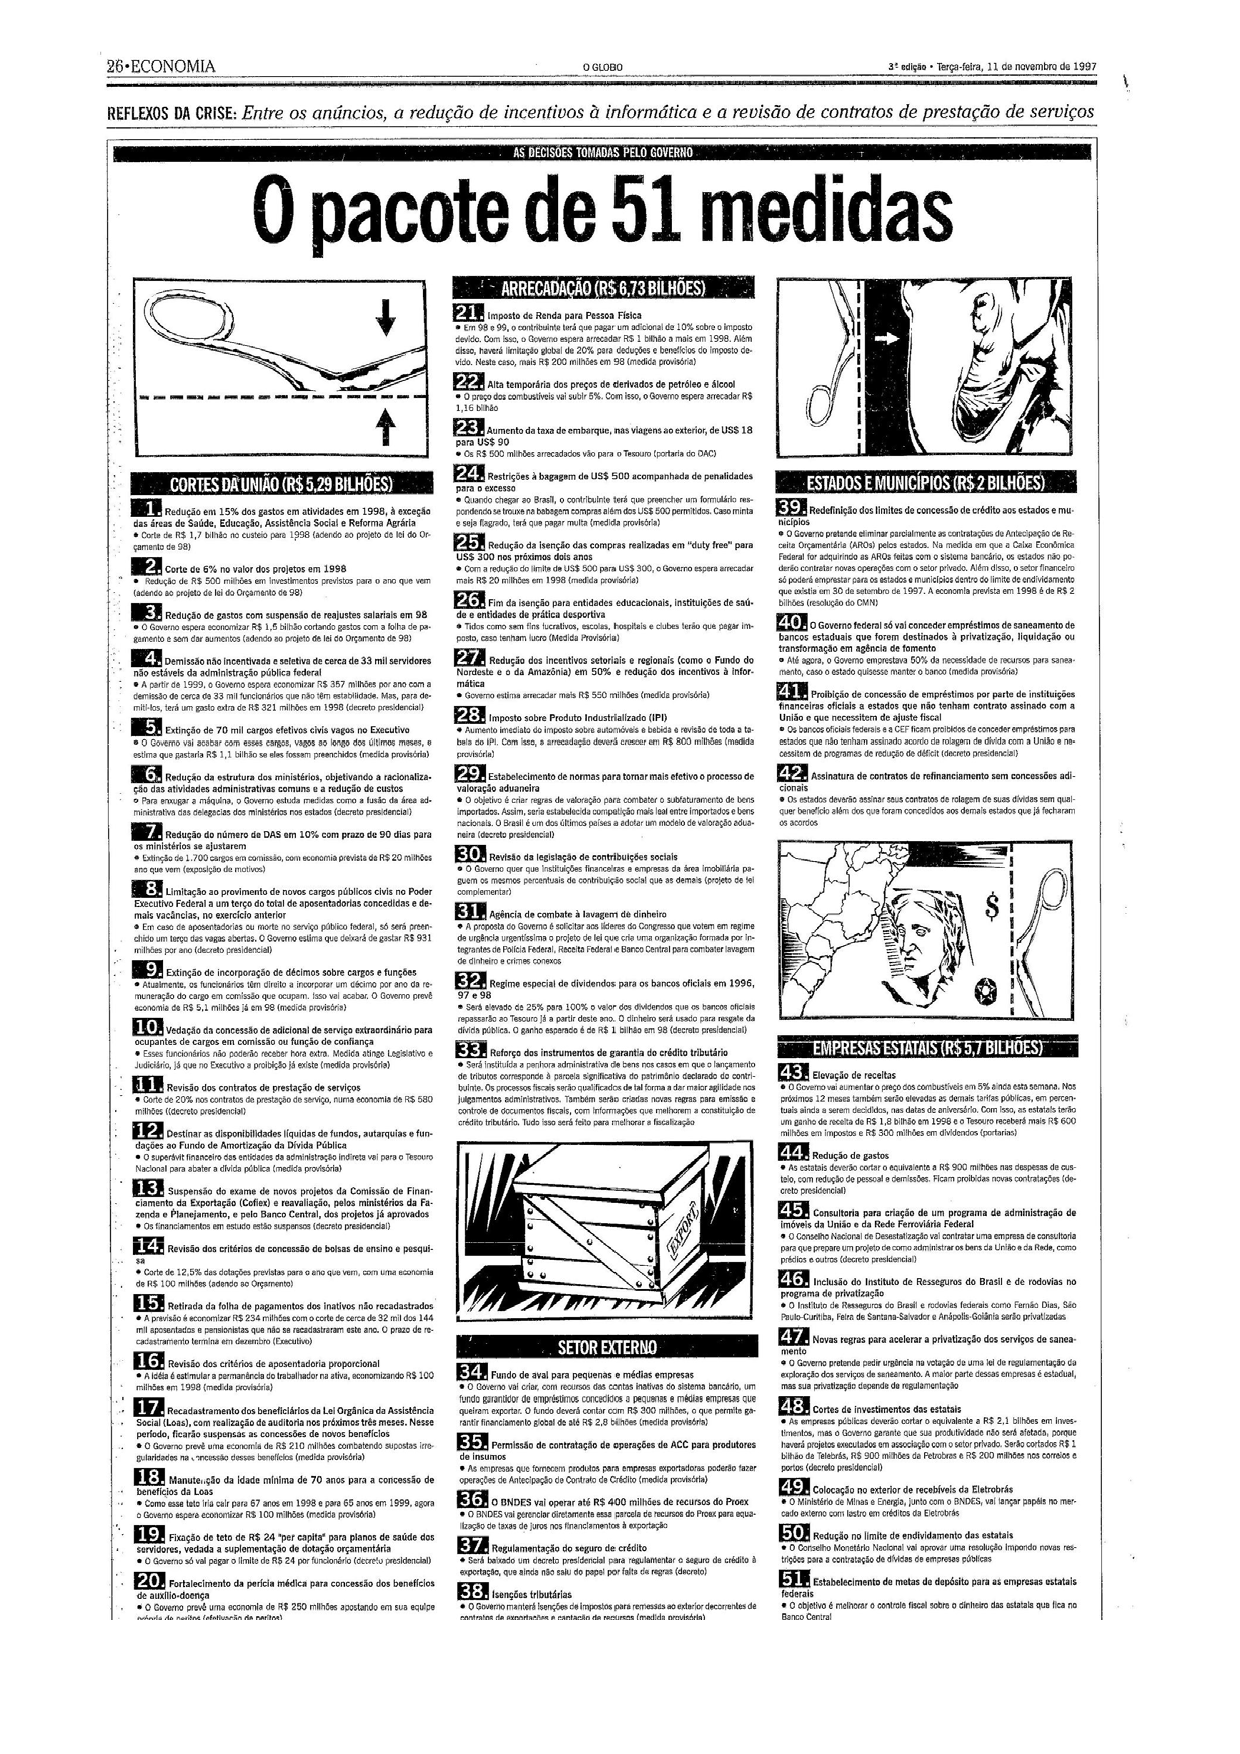
\includepdf[pages={1}]{./Jornais/Globo/as51medidasedit}

O pacote teria de ser negociado: no dia 12 de Novembro, a capa do O Globo j? anunciava que o Congresso j? sugeria um aumento da CPMF ao inv?s de um aumento no imposto de renda. A equipe econ?mica, afirmava o jornal, so aceitava o aumento da CPMF se a arrecada??o fosse desvinculada da sa?de. Afinal, n?o fosse assim, o aumento da CPMF n?o ajudaria a reduzir o d?ficit. 

Mas o presidente n?o aceitou a mudan?a e o pacote sofreria resist?ncia no congresso. Informava O Globo do dia 13 de Novembro que a bancada do PSDB, partido do presidente, era o ?nico a apoiar integralmente o pacote. Ant?nio Carlos Magalh?es, presidente do Senado e - normalmente - aliado do governo declarou que ``Ele (o presidente) manda l?, aqui mandamos n?s. A equipe econ?mica manda l?, aqui mandamos n?s". Do outro lado, Pedro Parente, na ?poca secret?rio-executivo do Minist?rio da Fazenda e futuro Ministro da Casa Civil - conhecido pela a habilidade diplom?tica - deixou de lado a diplomacia e disse que ``N?o estamos negociando nada. O conjunto de medidas ? este. ? o que achamos necess?rio. N?o distribu?mos benesses".

E, al?m do tiroteio com o Congresso, o governo rapidamente se veria envolvido em um conflito, dessa vez entre membros da equipe econ?mica. O ministro da Fazenda, Pedro Malan, disse a um jornal argentino que o Brasil podia fazer um acordo com o FMI. A declara??o viraria capa do O Globo de 18 de novembro, com a manchete ``Malan diz que acordo com FMI teria vantagens". No dia seguinte, era a vez de Gustavo Franco ser a manchete, da Folha de S?o Paulo: ``Acordo com FMI fere soberania, diz Franco". O Globo do mesmo dia ainda trazia o coment?rio de um dirigente do Banco Central dizendo que um acordo ``seria motivo para a demiss?o coletiva da diretoria"   

E no meio do tiroteio e da crise econ?mica, o governo conseguiria algumas vit?rias: a reforma administrativa foi aprovada na c?mara, o que traria uma economia de R\$5 bilh?es, segundo a manchete do O Globo de 20 de novembro. A capa trazia ainda outra boa not?cia: o Banco Central anunciava uma redu??o da taxa de juros, de 0,15 pontos percentuais. No dia 27 de Novembro, a capa do O Globo trazia outra vit?ria do governo: a quebra de estabilidade do servidor foi aprovada na c?mara.

Mas nem tudo eram flores, e no dia 29 de Novembro a Folha de S?o Paulo tinha como manchete ``FHC cede e muda pacote". O aumento do imposto de renda foi limitado. Em compensa??o, o imposto sobre renda fixa cresceu. O Globo

 

\subsection*{1998}
\addcontentsline{toc}{subsection}{1998}

\section{Conclus?o}

\begin{thebibliography}{16}
 \bibliographystyle{plainnat}

\bibitem[Grossmann(1998)]{Grossmann1998}
GROSSMANN, S. P.
\textbf{Desempenho das Contas P?blicas no Real: Uma an?lise da pol?tica fiscal no per?odo 1993-1997}
Rio de Janeiro, 1998. Disserta??o de Mestrado - Pontif?cia Universidade Cat?lica do Rio de Janeiro

\bibitem[Werneck(2014)]{Werneck2014}
WERNECK, R.L.F. \emph{Consolida??o da estabiliza??o e  reconstru??o institucional, 1995-2002} em 
ABREU, M. P. (org.). 
\textbf{A Ordem do Progresso: dois s?culos de pol?tica econ?mica no Brasil.}
2? edi??o.
Rio de Janeiro: Elsevier,
2014. p. 331-356

\bibitem[Giambiagi(2002)]{Giambiagi2002}
GIAMBIAGI, F.
\emph{Do D?ficit de Metas ?s Metas de D?ficit: a pol?tica fiscal do per?odo 1995-2002}
\textbf{PPE}, 
Abril de 2002. \\
Dispon?vel em: $\langle$http://www.ppe.ipea.gov.br/index.php/ppe/article/viewFile/277/214$\rangle$
Acesso em 12/12/2014

\bibitem[Franco(2005)]{Francoxxxx}
FRANCO, G.H.B.
\emph{Auge e decl?nio do inflacionismo no Brasil} em Fabio Giambiagi et al
\textbf{Economia brasileira contempor?nea}
$1^a$ edi??o
Rio de Janeiro: Elsevier, 
2005 p.258-283 


\end{thebibliography}

\end{document}